\chapter{Implementacja}

\section{Wprowadzenie do implementacji}

%TODO wrzucić listingi

Rozdział ten zawiera szczegóły implementacji aplikacji. Każdej scen poświęcono odpowiadający podrozdział wyjaśniający wykorzystane technologie, biblioteki oraz sposób komunikacji pomiędzy poszczególnymi elementami widoku. W projekcie zamieszczono kody funkcji realizujących najistotniejsze zadania.

\section{Struktura aplikacji}
Struktura projektu wykorzystuje domyślne ułożenie plików w systemie Unity. Jako główny folder służy folder \texttt{Assets}, zawiera on główne pliki projektowe: skrypty, tekstury, dźwięki, grafiki, prefaby(gotowe elementy często wykorzystywane w projekcie).

Struktura plików folderu \texttt{Scripts} podzielona została według ich celu. Każdy plik przypisany do sceny znajduje się w odpowiadającym mu folderze. Elementy pomocnicze jak np. skrypt pomocy kontekstowej, skrypt przycisku zamykania sceny znajdują się w folderze \texttt{Utility}.

Rysunek 4.1. pokazuje strukturę plików źródłowych projektu.
\begin{figure}[htb]
    \centering
	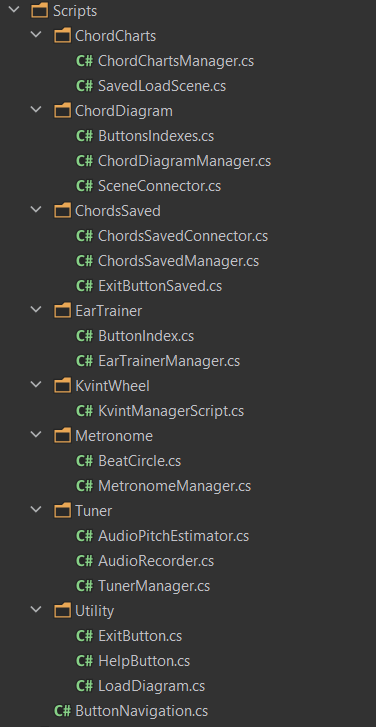
\includegraphics[width=0.45\linewidth]{rys04/StrukturaPlikow}
\end{figure}
% DONE: w rozdziale dobrze byłoby zamieścić opis struktury projektu. Ponieważ rozwijał Pan aplikację w środowisku UNITY, to środowisko narzuca trochę tę strukturę (parę uwag na ten temat też by się przydało). Strukturę projektu można pokazać robiąc zrzuty drzewa źródeł kodu.

% DONE: przydałoby się też opowiedzieć trochę o budowaniu aplikacji (testowe uruchomienia odbywają się w środowisku, aby można było uruchomić aplikację poza tym środowiskiem - coś trzeba przecież zrobić).
Aby na bieżąco analizować poprawność zaimplementowanych funkcji wykorzystywano wbudowaną w silnik Unity opcję \emph{play}, która umożliwia "odpalenie" jednej sceny, nie wymuszając przy tym budowania całej aplikacji od nowa. Po wykryciu zmian w skryptach aplikacja się przeładowuje i jest gotowa do użycia/przetestowania przez użytkownika.

\section{Implementacja elementów aplikacji}

\subsection{Stroik}

Głównymi elementami sceny sa przyciski służące do wyboru domniemanej nuty. W skład widoku wchodzi tez jej tytuł, informator odnośnie aktualnego poziomu nastrojenia instrumentu i przyciski odpowiedzialne za zmianę docelowego instrumentu. Do menadżera sceny przypięte zostały 3 skrypty realizujące logikę potrzebną do nagrania, przeanalizowania i wyświetlenia wyników analizy dźwięku. Nazwy tych skryptów to: \texttt{Audio Recorder} - skrypt odbierający dźwięk ze sceny, \texttt{Audio Pitch Estimator} - odpowiedzialny za analizę odebranego dźwięku, \texttt{Tuner Manager} - główny skrypt realizujący logikę sceny. 

Skrypt \texttt{Audio Recorder} zawiera dwa pola:
\begin{itemize}
    \item \texttt{audioSource} -- obiekt przechowujące odwołanie do wbudowanego w silnik Unity narzędzia \texttt{AudioSource}, umożliwiającego nagranie dźwięku,
    \item \texttt{duration} -- zmienna odpowiedzialna za ustalenie czasu, przez jaki mikrofon ma odbierać dźwięk z otoczenia.
\end{itemize}

Skrypt zawiera jedną funkcję \texttt{OnEnable}, która podczas uruchomienia zaczyna odbierać dźwięk dostarczany do mikrofonu. Skrypt \texttt{AudioPitchEstimator}, zaczerpnięty z repozytorium \cite{https://github.com/nakakq/AudioPitchEstimatorForUnity}, % TO DO: to nie jest poprawne cytowanie, proszę zrobić odpowiedni rekord w bib, a potem użyć jego klucza w \cite
służy do analizy odebranego dźwięku. Biblioteka zawiera poniżej wymienione zmienne, na które użytkownik może wpłynąć, aby dopasować narzędzie do swoich potrzeb.



\begin{itemize}
    \item \texttt{frequencyMin} -- minimalna częstotliwość, jaka ma być analizowana,
    \item \texttt{frequencyMax} -- maksymalna częstotliwość poddawana analizie,
    \item \texttt{harmonicsToUse} -- ilość harmonicznych jakie mają być brane pod uwagę, podczas ustalania końcowej częstotliwości odebranego dźwięku,
    \item \texttt{smoothingWidth} -- pasmo częstotliwości filtra wygładzającego widmo,
    \item \texttt{thresholdSRH} -- wartość graniczna decybeli, od której dźwięk ma być wzięty pod analizę.
\end{itemize}

Funkcją realizującą główną logikę działania jest metoda \texttt{Estimate}, wykonująca szybką transformatę Fouriera na odebranym dźwięku. Funkcja ta zwraca zmienną float \texttt{bestFreq}, będąca najlepszym możliwym według programu ,,trafieniem'', jeżeli chodzi o odebraną częstotliwość. Skrypt \texttt{TunerManager} odpowiedzialny za realizowanie logiki sceny, przechowuje odwołania do komponentów sceny: przyciski, pola tekstowe, obiekt \texttt{AudioSource}. W jego skład wchodzi 6 funkcji o nazwie \texttt{SetDesiredFrequency*}, przy czym każdemu z przycisków przypisany jest jeden jej odpowiednik, ustawiający parametry skryptu \texttt{AudioPitchEstimator}. Funkcją odpowiedzialną za logikę analizy dźwięku jest \texttt{EstimatePitch}, która korzysta ze skryptu \texttt{AudioPitchEstimator}, na tej podstawia ustawia wartości elementów tekstowych informujących użytkownika o poziomie nastrojenia instrumentu. 

\begin{lstlisting}[basicstyle=\footnotesize\ttfamily]
    public float Estimate(AudioSource audioSource)
    {
        var nyquistFreq = AudioSettings.outputSampleRate / 2.0f;

        // オーディオスペクトルを取得
        if (!audioSource.isPlaying) return float.NaN;
        audioSource.GetSpectrumData(spectrum, 0, FFTWindow.Hanning);

        // 振幅スペクトルの対数を計算
        // 以降のスペクトルはすべて対数振幅で扱う(ここは元論文と異なる)
        for (int i = 0; i < spectrumSize; i++)
        {
            // 振幅ゼロのとき-∞になってしまうので小さな値を足しておく
            specRaw[i] = Mathf.Log(spectrum[i] + 1e-9f);
        }

        // スペクトルの累積和(あとで使う)
        specCum[0] = 0;
        for (int i = 1; i < spectrumSize; i++)
        {
            specCum[i] = specCum[i - 1] + specRaw[i];
        }

        // 残差スペクトルを計算
        var halfRange = Mathf.RoundToInt((smoothingWidth / 2) / nyquistFreq * spectrumSize);
        for (int i = 0; i < spectrumSize; i++)
        {
            // スペクトルを滑らかに(累積和を使って移動平均)
            var indexUpper = Mathf.Min(i + halfRange, spectrumSize - 1);
            var indexLower = Mathf.Max(i - halfRange + 1, 0);
            var upper = specCum[indexUpper];
            var lower = specCum[indexLower];
            var smoothed = (upper - lower) / (indexUpper - indexLower);

            // 元のスペクトルから滑らかな成分を除去
            specRes[i] = specRaw[i] - smoothed;
        }

        // SRH (Summation of Residual Harmonics) のスコアを計算
        float bestFreq = 0, bestSRH = 0;
        for (int i = 0; i < outputResolution; i++)
        {
            var currentFreq = (float)i / (outputResolution - 1) * (frequencyMax - frequencyMin) + frequencyMin;

            // 現在の周波数におけるSRHのスコアを計算: 論文の式(1)
            var currentSRH = GetSpectrumAmplitude(specRes, currentFreq, nyquistFreq);
            for (int h = 2; h <= harmonicsToUse; h++)
            {
                // h倍の周波数では、信号が強いほど良い
                currentSRH += GetSpectrumAmplitude(specRes, currentFreq * h, nyquistFreq);

                // h-1倍 と h倍 の中間の周波数では、信号が強いほど悪い
                currentSRH -= GetSpectrumAmplitude(specRes, currentFreq * (h - 0.5f), nyquistFreq);
            }
            srh[i] = currentSRH;

            // スコアが最も大きい周波数を記録
            if (currentSRH > bestSRH)
            {
                bestFreq = currentFreq;
                bestSRH = currentSRH;
            }
        }

        // SRHのスコアが閾値に満たない → 明確な基本周波数が存在しないとみなす
        if (bestSRH < thresholdSRH) return float.NaN;

        return bestFreq;
    }
\end{lstlisting}

\begin{itemize}
    \item \texttt{Start} -- funkcja przypisująca przyciskom im działania w wypadku naciśnięcia.
    \item \texttt{ClearColor} -- funkcja pomocnicza, odpowiedzialna za ,,czyszczenie'' elementów graficznych sceny.
\end{itemize}

\subsection{Metronom}

Scena metronomu zawiera 9 przycisków służących do parametryzacji działania metronomu, umożliwiając zwiększenie tempa, zmianę metrum, zwiększanie lub zmniejszanie liczby taktów. Za logikę odpowiada menadżer sceny z przypiętym skryptem \texttt{MetronomeManager}, zawierający 10 pól obiektów przycisków, pole obiektu tekstowego i kilka zmiennych pomocniczych. Metronom realizowany jest za pomocą wizualizacji poszczególnych taktów za pomocą graficznych elementów w postaci "kółek", które dodawane sa do widoku dynamicznie w zależności od ustalonych przez użytkownika wartości. Funkcje jakie implementuje dany skrypt to:

\begin{itemize}
    \item \texttt{Start} -- funkcja odpowiadająca za ustawienie zmiennych, obiektów widoku. 
    \item \texttt{AddCircle} -- funkcja wykorzystywana do zwiększenia tempa.
    \item \texttt{DeleteCircle} -- funkcja wykorzystywana do zmniejszenia tempa.
    \item \texttt{RearrangeElements} -- funkcja stworzona do rozmieszczania ,,kółek'' taktów na ekranie.
    \item \texttt{StartMetronome} -- funkcja uaktywniająca metronom.
    \item \texttt{RecolorAll} -- funkcja uruchamiana podczas resetu metronomu, czyszcząca grafiki wizualizacji metronomu.
    \item \texttt{MetronomeCoroutine} -- osobny wątek odpowiedzialny za działanie metronomu, w czasie działania tej funkcji wybijane jest na ekranie tempo.
    \item \texttt{AddBpm} -- funkcja odpowiedzialna za zwiększenie tempa.
    \item \texttt{SubtractBpm} -- funkcja odpowiedzialna za zmniejszenie tempa.
\end{itemize}

Funkcja realizująca główną logikę sceny to \texttt{MetronomeCoroutine}, na bieżąco odgrywająca dźwięk oznaczający kolejny takt metronomu i zmieniająca kolory odpowiednich przycisków.
\begin{listing}[basicstyle=\footnotesize\ttfamily]
    IEnumerator MetronomeCoroutine()
    {
        
        float beatDuration = 60f / bpm;

        float noteDuration;
        noteDuration = beatDuration;

        int currentIndex = 0;
        int previousIndex = -1;

        while (true)
        {
            if (circles.Count > 0)
            {
                audioSource.Play();
                
           
                if (previousIndex != -1 && previousIndex < circles.Count)
                {
                    circles[previousIndex].GetComponent<BeatCircle>().changeColorWhite();
                }
                
                var currentCircle = circles[currentIndex].GetComponent<BeatCircle>();
                if (currentCircle.imgComponent.color == Color.black)
                {
                    currentCircle.changeColorWhite();
                }
                else
                {
                    currentCircle.changeColorBlack();
                }

                previousIndex = currentIndex;
                currentIndex = (currentIndex + 1) % circles.Count;
            }
            
            yield return new WaitForSeconds(noteDuration);
        }
    }
\end{listing}
\subsection{Księga akordów}

Scena księgi akordów zawiera element graficzny reprezentujący aktualnie wybrany akord gitarowy, przyciski umożliwiające wybór docelowego akordu, elementy graficzne ułatwiające nawigację po widoku sceny. Funkcje wchodzące w skład skryptu menadżera sceny nazwanego \texttt{ChordChartsManager} to:

\begin{itemize}
    \item \texttt{Start} -- funkcja odpowiedzialna za przygotowanie potrzebnych elementów sceny. Przypisuje grafiki akordów z pomocniczej listy Chords do listy głównej ch. Ustawia wartości zmiennych noteIterator, variantIterator z wartości przechowywanych w skrypcie SceneConnector, łączącej scenę księgi akordów z widokiem wszystkich akordów w postaci diagramu. Przypisuje ona funkcje do odpowiednich przycisków i resetuje wartości obiektów tekstowych.
    \item \texttt{noteIncrement} -- funkcja przypisana do przycisku, odpowiedzialna za zmianę nuty akordu.
    \item \texttt{noteDecrement} -- funkcja przypisana do przycisku, odpowiedzialna za zmianę nuty akordu.
    \item \texttt{variantIncrement} -- funkcja przypisana do przycisku, odpowiedzialna za zmianę wariacji akordu.
    \item \texttt{variantDecrement} -- funkcja przypisana do przycisku, odpowiedzialna za zmianę wariacji akordu.
    \item \texttt{ChangeVariantText} -- funkcja odpowiedzialna za zmianę przypisanej wartości obiektu tekstowego sceny, wykorzystywana w momencie zmiany wariacji akordu.
    \item \texttt{ChangeNoteText} -- funkcja odpowiedzialna za zmianę przypisanej wartości obiektu tekstowego sceny, wykorzystywana w momencie zmiany nuty akordu.
    \item \texttt{ChangeChord} -- funkcja odpowiedzialna za zmianę aktualnie wyświetlanego akordu, zmienia przypisaną grafikę obiektu Image sceny.
\end{itemize}

\subsection{Trening słuchu}

Scena treningu słuchu zawiera przycisk odpowiedzialny za odegranie dźwięku, który następnie ma zostać odgadnięty przez użytkownika za pomocą jednego z 12 przycisków obecnych na scenie. W skład sceny wchodzą dwa skrypty: \texttt{EarTrainerManager} -- przypisany do menadżera sceny realizujący główną logikę sceny oraz \texttt{ButtonIndex} -- skrypt pomocniczy przypisany do każdego z 12 przycisków odpowiedzialnych za udzielenie odpowiedzi. Funkcje wchodzące w skład głównego skryptu to:
\begin{itemize}
    \item \texttt{Start} -- funkcja przypisująca obiekt \texttt{audioSource}, odpowiedzialny za odgrywanie dźwięków. Ustawia ona również funkcję \texttt{PlayRandomNote} do przycisku \texttt{playNoteButton}. Dodatkowo przypisuje ona funkcję \texttt{NoteGuessed} do każdego z przycisków odpowiedzialnych za odpowiedź.
    \item \texttt{PlayRandomNote} -- funkcja odpowiedzialna za odegranie losowego dźwięku po naciśnięciu przycisku \texttt{playNoteButton}. Ustawia ona odpowiedni index dla odegranej nuty, wykorzystywany następnie podczas zweryfikowania odpowiedzi podanej przez użytkownika.
    \item \texttt{NoteGuessed} -- funkcja weryfikująca odpowiedź użytkownika, wykorzystywana po naciśnięciu jednego z 12 przycisków odpowiedzi. Ustawia ona obiekty tekstowe sceny, w zależności od tego czy odpowiedź była poprawna, czy też nie. 
\end{itemize}

Skrypt pomocniczy przechowuje jedynie jedną zmienną, wykorzystywaną w momencie weryfikacji odpowiedzi udzielonej przez użytkownika, jest nią: \texttt{buttonNumber}.

\subsection{Koło kwintowe}

Scena koła kwintowego zawiera 24 przyciski, każdemu z nich przypisana została odpowiednia nuta. W skrypcie menadżera sceny utworzone zostały dwie listy, przechowujące przyciski koła zewnętrznego oraz koła wewnętrznego. Skrypt zawiera w sobie 6 funkcji:

\begin{itemize}
\item \texttt{Start} -- funkcja używana podczas tworzenia obiektu, służy ona przygotowaniu wszystkich przycisków oraz przypisania im działania przy ich naciśnięciu, w tym przypadku przypisuje ich działanie do funkcji \texttt{DisplayScale}
\item \texttt{DisplayScale} -- funkcja odpowiedzialna jest ona za wyświetlenie skali majorowej, oraz 3 akordów minorowych pasujących do wybranej przez użytkownika nuty. 
\item \texttt{GetColorTin}t -- funkcja pomocnicza generująca kolejne odcienie kolorów, dla funkcji \texttt{DisplayScale}.
\item \texttt{GetMajorScaleIndices} -- funkcja pomocnicza generująca interwały kolejnych nut w skali majorowej.
\item \texttt{ChangeButtonColor} -- funkcja pomocnicza odpowiedzialna za zmianę koloru odpowiedniego przycisku.
\item \texttt{ClearColors} -- funkcja pomocnicza czyszcząca kolory wszystkich przycisków.
\end{itemize}

